\documentclass[11pt,a4paper]{article}
\usepackage[utf8]{inputenc}
\IfFileExists{lmodern.sty}{\usepackage[T1]{fontenc}\usepackage{lmodern}}{}
\usepackage[margin=2.5cm]{geometry}
\usepackage{booktabs,tabularx,longtable,array}
\usepackage{graphicx}
\usepackage{amssymb}
\usepackage{enumitem}
\usepackage[round]{natbib}
\usepackage{xcolor}
\usepackage[colorlinks=true,linkcolor=blue!50!black,citecolor=blue!50!black,urlcolor=blue!50!black]{hyperref}
\setlist{nosep,leftmargin=*}
\newcolumntype{L}{>{\raggedright\arraybackslash}X}
\graphicspath{{figures/}}
\emergencystretch=2em
% generated by paper/code/assets.py -- do not edit
\newcommand{\whMeets}{5}
\newcommand{\whPartial}{8}
\newcommand{\dMeets}{1}
\newcommand{\dPartial}{9}
\newcommand{\unMeets}{0}
\newcommand{\unPartial}{4}
\newcommand{\pilotPaths}{13}
\newcommand{\cheapUChars}{7{,}937}
\newcommand{\cheapUShare}{27}
\newcommand{\compUChars}{9{,}149}
\newcommand{\compDChars}{4{,}747}
\newcommand{\compUOverCheap}{15}
\newcommand{\compliantResp}{2{,}834}
\newcommand{\compliantFilled}{2{,}929}
\newcommand{\dMetaShareMin}{46}
\newcommand{\dMetaShareMax}{50}
\newcommand{\unPilotShareMin}{19}
\newcommand{\unPilotShareMax}{21}
\newcommand{\whDtpChars}{7{,}350}
\newcommand{\whDtpShare}{67}
\newcommand{\nSeries}{34}
\newcommand{\nQuestions}{58}
\newcommand{\nQuestionsD}{24}
\newcommand{\nAnswers}{140}
\newcommand{\callsUsed}{325}
\newcommand{\answeredBoth}{51}
\newcommand{\whShareMin}{46}
\newcommand{\whShareMax}{70}
\newcommand{\unShareMax}{21}
\newcommand{\dShareMin}{20}
\newcommand{\dShareMax}{29}
\newcommand{\unCheaper}{43}
\newcommand{\medWh}{13.4}
\newcommand{\medUn}{8.9}
\newcommand{\medD}{4.2}
\newcommand{\discUn}{94}
\newcommand{\discWh}{67}
\newcommand{\structWh}{10}
\newcommand{\dataUn}{6}
\newcommand{\dataWh}{22}
\newcommand{\dataCallWh}{1.9}
\newcommand{\dataCallUn}{0.6}
\newcommand{\searchWh}{9.6}
\newcommand{\unMaxChars}{128}
\newcommand{\dFound}{4}
\newcommand{\dSeries}{14}
\newcommand{\braAns}{10}
\newcommand{\somAns}{7}
\newcommand{\braQ}{12}
\newcommand{\somQ}{12}
\newcommand{\noDataWh}{12.6}
\newcommand{\noDataUn}{0.6}
\newcommand{\rhoUn}{0.36}
\newcommand{\rhoWh}{0.60}
\newcommand{\unAgree}{41}
\newcommand{\unCommon}{51}
\newcommand{\unLatSame}{37}
\newcommand{\unLatEarlier}{11}
\newcommand{\unLatLater}{3}
\newcommand{\dAgree}{12}
\newcommand{\dCommon}{19}
\newcommand{\dLatSame}{14}
\newcommand{\dLatEarlier}{6}
\newcommand{\dLatN}{22}
\newcommand{\sessions}{96}
\newcommand{\valuesRep}{1{,}953}
\newcommand{\valuesOK}{1{,}952}
\newcommand{\valuesGrounded}{1{,}953}
\newcommand{\boundsRep}{290}
\newcommand{\boundsOK}{290}
\newcommand{\refYears}{246}
\newcommand{\cellsSameVal}{11}
\newcommand{\cellsSameSeries}{9}
\newcommand{\cells}{12}
\newcommand{\metaSpread}{5}
\newcommand{\repSeries}{12}
\newcommand{\repCalls}{3}
\newcommand{\repMax}{22}
\newcommand{\repMed}{12}
\newcommand{\opusEffort}{25}
\newcommand{\haikuRatio}{1.8}
\newcommand{\sigs}{68}
\newcommand{\sigsSame}{67}
\newcommand{\unSigs}{18}
\newcommand{\unByteDiff}{11}
\newcommand{\sentPerRecv}{356}
\newcommand{\baseShare}{84}
\newcommand{\cacheShare}{88}
\newcommand{\baseTok}{97{,}000}
\newcommand{\schemaUn}{15{,}000}
\newcommand{\schemaWh}{20{,}000}
\newcommand{\schemaD}{22{,}000}
\newcommand{\defMin}{70}
\newcommand{\defMax}{80}
\newcommand{\respMin}{17}
\newcommand{\respMax}{33}
\newcommand{\reqMin}{4}
\newcommand{\reqMax}{6}
\newcommand{\charsUnNoFile}{8.1}
\newcommand{\charsWhAg}{16.6}
\newcommand{\charsDAg}{27.3}
\newcommand{\instrChars}{12{,}000}
\newcommand{\dMetaChars}{18{,}600}
\newcommand{\tsCalls}{54}
\newcommand{\qdCalls}{17}
\newcommand{\oversizedM}{1.3}
\newcommand{\recvHaikuMedium}{2{,}860}
\newcommand{\callsHaikuMedium}{62}
\newcommand{\sentHaikuMedium}{655}
\newcommand{\recvSonnetLow}{1{,}483}
\newcommand{\callsSonnetLow}{47}
\newcommand{\sentSonnetLow}{587}
\newcommand{\recvSonnetMedium}{1{,}569}
\newcommand{\callsSonnetMedium}{46}
\newcommand{\sentSonnetMedium}{588}
\newcommand{\recvSonnetHigh}{1{,}805}
\newcommand{\callsSonnetHigh}{57}
\newcommand{\sentSonnetHigh}{643}
\newcommand{\recvOpusLow}{1{,}308}
\newcommand{\callsOpusLow}{38}
\newcommand{\sentOpusLow}{551}
\newcommand{\recvOpusMedium}{1{,}631}
\newcommand{\callsOpusMedium}{51}
\newcommand{\sentOpusMedium}{639}
\newcommand{\recvOpusHigh}{1{,}823}
\newcommand{\callsOpusHigh}{57}
\newcommand{\sentOpusHigh}{690}
\newcommand{\recvOpusMediumRepeat}{1{,}608}
\newcommand{\callsOpusMediumRepeat}{47}
\newcommand{\sentOpusMediumRepeat}{563}
\newcommand{\tShareUnK}{51}
\newcommand{\tShareUnN}{51}
\newcommand{\tShareUnP}{$<10^{-12}$}
\newcommand{\tCostUnK}{43}
\newcommand{\tCostUnN}{58}
\newcommand{\tCostUnP}{0.0003}
\newcommand{\tShareDK}{22}
\newcommand{\tShareDN}{22}
\newcommand{\tShareDP}{$<10^{-6}$}
\newcommand{\tCostDK}{22}
\newcommand{\tCostDN}{24}
\newcommand{\tCostDP}{$<10^{-4}$}
\newcommand{\effOpusK}{12}
\newcommand{\effSonnetK}{12}
\newcommand{\effN}{12}
\newcommand{\effOpusRecvK}{12}
\newcommand{\effSonnetRecvK}{12}
\newcommand{\effP}{0.0005}
\newcommand{\effOpusPct}{33}
\newcommand{\effSonnetPct}{6}
\newcommand{\effOpusRecvPct}{38}
\newcommand{\effSonnetRecvPct}{21}
\newcommand{\repCellMed}{2}
\newcommand{\repCellMax}{22}
\newcommand{\errBoundSess}{3.1}
\newcommand{\errBoundVal}{0.15}
\newcommand{\wrongSessions}{0}


\title{Metadata, cost and accuracy of official statistics served to AI agents:\\ evidence from three MCP servers}
\author{Jo\~ao Pedro Azevedo\\ UNICEF, Office of Strategy and Evidence, Data and Analytics\thanks{Working draft. Every number, table and figure is generated from the replication package that accompanies this paper; see the Reproducibility section.}}
\date{27 October 2026}

\begin{document}
\maketitle

\begin{abstract}
\noindent AI agents increasingly reach official statistics through Model Context Protocol (MCP) servers rather than through portals or application programming interfaces. A value that reaches an agent without its source, status, uncertainty or release cannot be attributed, dated or interpreted correctly. This paper proposes a minimum metadata standard of fifteen elements for MCP servers that republish official statistics. It scores three public servers against it: the UNICEF SDMX data warehouse MCP, the UN System Data Commons (UN DC) and World Bank Data360. It then measures what answering a question costs on each. Three designs are used: a scripted pilot on two Nigerian series; a pre-registered benchmark of \nSeries{} randomly drawn series across 17 sectors and three countries (\nAnswers{} answers, \callsUsed{} calls); and an agentic benchmark of \sessions{} sessions across seven model and effort settings. The warehouse delivers \whShareMin--\whShareMax\% of the standard on every question it answers, against at most \unShareMax\% for UN DC and \dShareMin--\dShareMax\% for Data360. Compliance is cheap, because the metadata travels in the data call, which accounts for \dataUn--\dataWh\% of characters on UN DC and the warehouse; searching for the series accounts for \discWh--\discUn\%. Across models and effort levels, every reported value for a year the warehouse holds (\valuesOK{} of \valuesRep{}) matched it, and all \valuesGrounded{} appeared in the servers' own responses. Higher effort raised cost, not accuracy. In agentic use, the tool definitions a server loads into every request cost more tokens than its data responses. For an official UNICEF MCP, the levers are a compact search, a short tool list, and one data call that carries the fifteen elements.

\medskip\noindent\textbf{Keywords:} official statistics; metadata; SDMX; Model Context Protocol; AI agents; data dissemination.
\end{abstract}

% ======================================================================
\section{Introduction}\label{sec:intro}

When an analyst asks an AI assistant for Nigeria's under-five mortality rate, the number usually no longer comes from a portal, a PDF or a download. An agent calls a tool exposed by an MCP server, reads the response and writes an answer. Whatever the server leaves out of that response, the answer cannot contain: who produced the estimate, which release it belongs to, whether it was modelled or reported, and how uncertain it is. For official statistics, whose value rests on provenance and method as much as on the number, this is a new and largely unexamined channel.

This paper asks two questions. First, what metadata must a server return with each value for an agent to reproduce, attribute, date and interpret it, and how far do current servers meet that bar? Second, what does it cost, in characters and tokens, to answer a statistical question through each server, and does that cost depend on the metadata, on the server's design, or on the model that drives the agent?

We answer them for three public MCP servers that republish UNICEF's child-related indicators: the UNICEF SDMX data warehouse MCP (sdmx-mcp 1.2.214), the UN System Data Commons MCP, and the World Bank Data360 MCP. We propose a minimum standard of fifteen elements, each reusing an attribute already defined by SDMX \citep{sdmx}, the SDG data structure definition \citep{unsd2019} or the UNICEF warehouse. We score the three servers against it, and run three benchmarks of increasing realism.

We find four things.
\begin{itemize}
\item \textbf{Coverage of the standard ranks the servers consistently.} The warehouse delivers \whShareMin--\whShareMax\% of the standard wherever it answers, against at most \unShareMax\% for UN DC and \dShareMin--\dShareMax\% for Data360.
\item \textbf{Compliance is not a cost problem.} The metadata travels in the data call, the cheap part of any answer; searching for the right series accounts for \discWh\% of the warehouse's characters and \discUn\% of UN DC's.
\item \textbf{Accuracy did not depend on the model or the effort level.} Every value agents reported for a year the warehouse holds (\valuesOK{} of \valuesRep{}) matched it, and all \valuesGrounded{} appeared in the servers' own responses. Higher effort bought more calls, not better answers.
\item \textbf{The tool definitions a server loads cost more than its data.} In agentic use they are re-sent with every request and add \defMin{},000--\defMax{},000 tokens per question on average; all data responses and reasoning together add \respMin{},000--\respMax{},000.
\end{itemize}

Section~\ref{sec:motivation} motivates the problem. Section~\ref{sec:method} sets out the standard, the scoring and the cost measures. Section~\ref{sec:data} describes the servers, samples and data recorded. Section~\ref{sec:results} presents results, Section~\ref{sec:policy} draws policy implications and Section~\ref{sec:final} concludes with limitations.

% ======================================================================
\section{Motivation}\label{sec:motivation}

\paragraph{An official statistic is a value plus its metadata.} The same national under-five mortality rate can be a modelled UN IGME estimate with a 90 per cent uncertainty interval \citep{igme2025}, or a direct estimate from one survey round. A coverage rate can come from the latest WHO/UNICEF revision or from the one before it. The international statistical system has spent two decades codifying how this information travels between agencies. The SDG data structure definition makes the unit, unit multiplier and observation status mandatory, and defines source detail, time detail, bounds and observation comments \citep{unsd2019}. The Statistical Commission's guidelines on data flows and global data reporting set out how data and metadata should pass between national systems and custodian agencies \citep{unsc2018}, and the CCSA principles ask for credit to the original source \citep{ccsa2016}. None of this yet reaches the channel through which AI agents now read the data.

\paragraph{Republishing multiplies the risk of loss.} A UNICEF value may reach an agent directly from the warehouse, or through a republisher that copied it from the SDG Global Database or from a World Bank collection. At each hop attributes can be dropped, codes re-mapped and releases fall out of date. Our earlier comparisons found concrete cases of each: UN DC attributes every UNICEF facet to ``United Nations''; Data360 credits UNICEF on 65 of 117 matched series; and both still served Nigeria's pre-revision DTP3 coverage for 2021--2024 (61, 59, 67, 67), where the warehouse, on the WUENIC 2025 revision, has 50, 55, 63 and 63. An agent cannot detect any of these from the response alone.

\paragraph{Cost shapes what agents can use.} Agents are billed and limited by tokens. A server that returns 30,000 characters where 3,000 would do makes every answer slower and dearer, crowds the model's context, and may push the agent to stop early or to skip a metadata call. A standard that made responses much longer would not be adopted; a server that is cheap only because it drops metadata is not a good server.

\paragraph{There is no standard yet.} The MCP specification defines how a tool declares an output schema and returns structured content, but not what a statistical response should contain \citep{mcp2026}. UNICEF is preparing an official MCP server for its data, and the UN system is building shared infrastructure through the UN System Data Commons under UN80 Workstream 16. Both need an agreed minimum and evidence on what it costs.

% ======================================================================
\section{Methodology}\label{sec:method}

\subsection{A minimum metadata standard}

An element enters the standard only if its absence caused a documented failure in our comparisons of the three servers against the warehouse, and each reuses an attribute that SDMX, the SDG data structure definition or the UNICEF warehouse already defines. Elements attach at three levels: R elements once per response, S elements once per series, and O elements per observation, only when non-empty. Twelve are required in every response; three (marked $^{*}$) whenever the custodian publishes them (Table~\ref{tab:standard}).

\begin{table}[htbp]\centering\small
\caption{The minimum metadata standard}\label{tab:standard}
\begin{tabularx}{\textwidth}{@{}l>{\raggedright\arraybackslash}p{3.3cm}LL@{}}
\toprule
ID & Element & What it must hold & Reuses \\ \midrule
\csname @@input\endcsname generated/tab1_standard.tex 
\bottomrule
\multicolumn{4}{@{}l}{\footnotesize $^{*}$ Required whenever the custodian publishes it.}
\end{tabularx}
\end{table}

Seven carriage rules accompany the elements: (1) pass every element through and never drop one; (2) inline what interpretation needs and link the rest; (3) send header fields once per series and per-observation fields only where they vary; (4) send every coded field as code and label; (5) declare every default the server applied; (6) return values as published, without extra rounding or silent scaling; (7) declare the response schema through MCP's \texttt{outputSchema}.

\subsection{Scoring}
Each answer is scored element by element as \emph{meets} (1 point), \emph{partial} (0.5) or \emph{missing} (0). Partial means incomplete, uneven across flows, or available only through a separate call. Elements the custodian does not publish for that series and country are not applicable. The \emph{share of the standard delivered} is points divided by applicable elements. The automated scoring reproduces all ten hand-scored pilot paths element by element.

\subsection{Cost}
Cost is measured in characters of every MCP response, counted exactly from the agents' session transcripts (oversized responses from the copy the client saved), and, in the agentic benchmark, in tokens: the usage the API reported for each request. Tokens sent are input plus cache-creation plus cache-read tokens, summed over requests; tokens received are output tokens, thinking included. Tokens sent are decomposed into the \emph{baseline} (the first request, i.e.\ the client's own instructions and tool list, times the number of requests), \emph{tool definitions} (the jump in context when the server's tools load, times later requests) and the \emph{remainder} (responses and reasoning carried forward). A transcript repeats the usage of one API response on each of its content blocks, so usage is counted once per message identifier.

\subsection{Frontier, accuracy and grounding}
A way of answering is on the \emph{efficiency frontier} if no other way delivers at least the same share of the standard for fewer characters. A value is \emph{correct} if it is within the larger of 0.5\% relative error and the rounding unit of the value reported (0.51 for integers, 0.051 otherwise) of the warehouse value for that year. A number is \emph{grounded} if it appears in the server's responses in that session, verbatim or rounded to the precision reported.

\subsection{Three benchmark designs}
\begin{table}[htbp]\centering\small
\caption{Benchmark designs}\label{tab:designs}
\begin{tabularx}{\textwidth}{@{}>{\raggedright\arraybackslash}p{2.2cm}>{\raggedright\arraybackslash}p{3.4cm}>{\raggedright\arraybackslash}p{2.4cm}LL@{}}
\toprule
Design & Questions & Who chooses the calls & Measures & Purpose \\ \midrule
Pilot & 2 series, Nigeria; \pilotPaths{} paths & analyst, scripted & characters, share & build and calibrate the scoring; first frontier \\
Sector and country & \nSeries{} series $\times$ up to 3 countries; \nAnswers{} answers & fixed path per server, pre-registered & characters by component, share, discovery, agreement & test whether the pilot generalises \\
Model and effort & 4 series, Nigeria $\times$ 3 servers $\times$ 8 runs; \sessions{} sessions & the agent & tokens sent and received, calls, accuracy, grounding, stability & separate the server from the model \\
\bottomrule
\end{tabularx}
\end{table}

% ======================================================================
\section{Data}\label{sec:data}

\paragraph{Servers.} All three servers were queried on 26--27 October 2026 through their public MCP endpoints. The \emph{UNICEF SDMX warehouse MCP} (sdmx-mcp 1.2.214) reads the warehouse's public SDMX REST API (\url{https://sdmx.data.unicef.org}), which holds UNICEF's 41 dataflows, through 31 tools for discovery, structure and data. The \emph{UN System Data Commons MCP} serves a knowledge graph of UN-system statistics, including UNICEF series taken from the SDG Global Database and from UNICEF directly, through six tools and an instruction file it asks agents to read first. The \emph{World Bank Data360 MCP} serves World Bank databases (among them WDI, Health, Nutrition and Population, and the Human Capital Project), which republish many UNICEF series under World Bank codes, through 16 tools, with data and metadata in separate calls.

\paragraph{Pilot.} Two questions for Nigeria, 2000--2025: the under-five mortality rate (UN IGME) and DTP3 coverage (WUENIC), each answered by every reasonable path on each server, with and without a separate metadata call. Data360 was first queried from 1960 and 1980, which made its responses 2.3 and 1.6 times longer, so it was re-run on the same window; both runs are kept and the first is flagged.

\paragraph{Sector and country sample.} The frame is the 210 UNICEF indicator codes in UN DC whose series maps to a warehouse series with Nigerian data. Codes are stratified by UN DC's 17 UNICEF sector groups and, within each, ranked by their number of UN DC variables and split into lower and upper halves. One code is drawn per stratum with a fixed seed (20261027), giving \nSeries{} series. All are asked for Nigeria, and twelve drawn at random also for Brazil and data-sparse Somalia: \nQuestions{} questions on the warehouse and UN DC, and \nQuestionsD{} on Data360 for the \dSeries{} series it carries. Each server follows one path fixed in advance; discovery uses the custodian's indicator name, with one retry using UN DC's name; the data call always uses the target identifier, so retrieval cost is measured even when discovery fails. Protocol and sample were saved before the first call; agents executed \callsUsed{} calls used in the analysis, and every response is saved verbatim.

\paragraph{Model and effort panel.} Four questions for Nigeria, 2000--2025, chosen because all three servers hold the series and its values agree with the warehouse: the under-five mortality rate (UN IGME), the maternal mortality ratio (MMEIG), the population using at least basic drinking water services (JMP), and women aged 15--49 with four or more antenatal care visits (UNICEF household-survey database). The warehouse values are the reference. Each agent received the same prompt, could use only one server (no web search, files or prior knowledge), and had to answer in a fixed JSON form, returning null for anything the server did not give it. Seven settings were run --- Claude Haiku 5.5 at medium effort, and Claude Sonnet 5.5 and Claude Opus 5.5 at low, medium and high effort --- plus a repeat of Opus at medium effort: \sessions{} sessions. Claude Fable 5.1 was planned, but all 12 of its sessions were refused because the account had no usage credits for it.

% ======================================================================
\section{Results}\label{sec:results}

\subsection{How far the servers meet the standard}
The warehouse MCP meets \whMeets{} of the 15 elements and partly meets \whPartial{}; Data360 meets \dMeets{} and partly meets \dPartial{}, mostly through its separate metadata call; UN DC meets \unMeets{} and partly meets \unPartial{} (Figure~\ref{fig:compliance}, Table~\ref{tab:compliance}). The ranking follows what each server passes through: the warehouse publishes most of what the standard needs, unevenly across its 41 flows; Data360 holds rich series metadata but keeps it apart from the data; UN DC drops every observation-level attribute, so even where it copies warehouse values it loses the bounds, status, sources and notes attached to them. No server meets the retrieval stamp (R2) or licence with citation (S7), the two elements any server can add without touching its data.

\begin{figure}[htbp]\centering
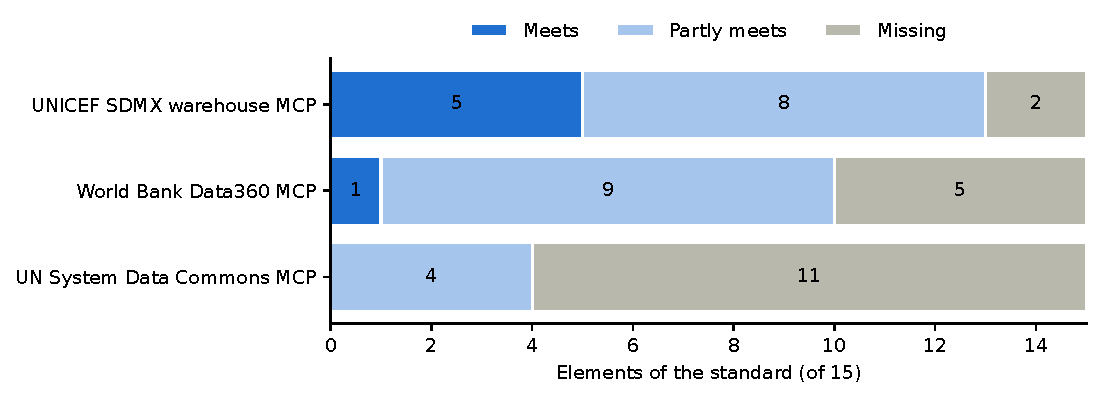
\includegraphics[width=\textwidth]{fig1_compliance.pdf}
\caption{Elements of the standard met in a data response, by server. Meets: present in the response to a data query; partly: incomplete, uneven across flows, or only via a separate call.}\label{fig:compliance}
\end{figure}

\begin{table}[htbp]\centering\small
\caption{Element-by-element status (M = meets, P = partly meets, -- = missing), with the evidence for the warehouse}\label{tab:compliance}
\begin{tabularx}{\textwidth}{@{}>{\raggedright\arraybackslash}p{4.2cm}cccL@{}}
\toprule
Element & Warehouse & UN DC & Data360 & Warehouse evidence \\ \midrule
\csname @@input\endcsname generated/tab3_compliance.tex 
\bottomrule
\end{tabularx}
\end{table}

\subsection{The pilot frontier}
On the two pilot questions the cheapest answer delivers between a quarter and two-thirds of the standard, and a compliant answer would cost about the same (Figure~\ref{fig:pilot}). For under-five mortality, the cheapest answer is Data360's data call: \cheapUChars{} characters and \cheapUShare\% of the standard. For DTP3, the warehouse's two-call answer (\whDtpChars{} characters, \whDtpShare\%) is on the frontier. Adding its metadata call lifts Data360 to \dMetaShareMin--\dMetaShareMax\% at a cost of 16--19 thousand extra characters, more than half of them lists of countries, regions and years; UN DC stays at \unPilotShareMin--\unPilotShareMax\% whether or not it adds its own metadata call.

A standard-compliant response, built from the warehouse's own values and attributes with unpublished fields left as placeholders, takes \compliantResp{} characters for 25 years of under-five mortality (\compliantFilled{} once the placeholders are filled at typical lengths), fewer than the warehouse's current data response. With the warehouse's discovery call, it costs \compUChars{} and \compDChars{} characters for the two questions: about \compUOverCheap\% more than the cheapest answer measured today for under-five mortality, and less than any answer measured for DTP3, for 100\% of the standard.

\begin{figure}[htbp]\centering
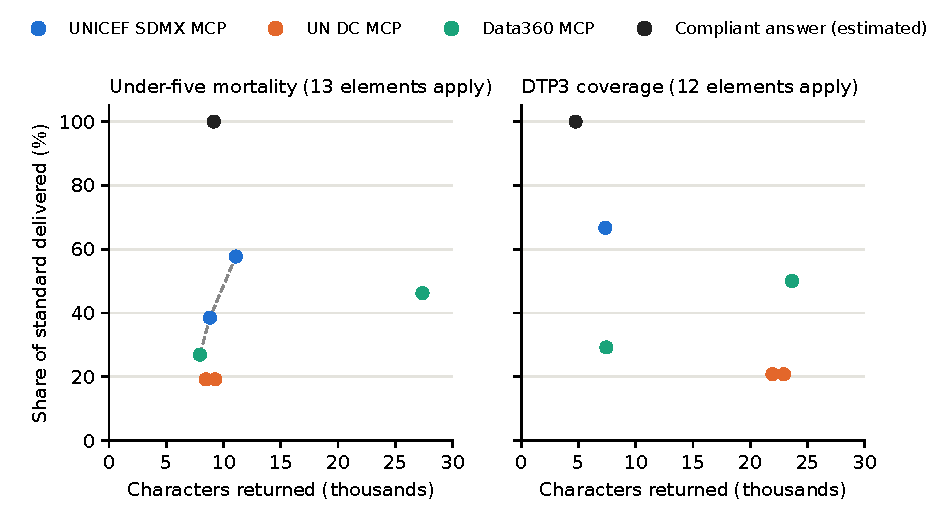
\includegraphics[width=\textwidth]{fig2_pilot_frontier.pdf}
\caption{The pilot frontier: characters returned against share of the standard delivered, Nigeria 2000--2025. Dashed line: measured frontier.}\label{fig:pilot}
\end{figure}

\subsection{Across sectors and countries}
The pre-registered benchmark confirms the ranking on the standard but overturns the ranking on cost (Figure~\ref{fig:scatter}). On all \answeredBoth{} questions that both servers answered, the warehouse delivered more of the standard than UN DC: \whShareMin--\whShareMax\% against at most \unShareMax\%. Data360 delivered \dShareMin--\dShareMax\%. But UN DC's answer was cheaper than the warehouse's on \unCheaper{} of \nQuestions{} questions. Median characters per question were \medWh{} thousand for the warehouse, \medUn{} thousand for UN DC and \medD{} thousand for Data360. The pilot questions had flattered the warehouse: its search returns a median \searchWh{} thousand characters for a custodian indicator name.

\begin{figure}[htbp]\centering
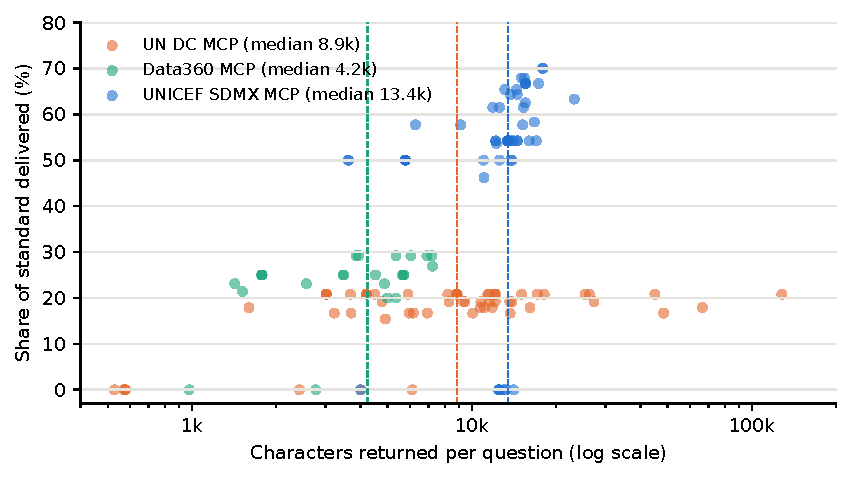
\includegraphics[width=\textwidth]{fig3_sector_scatter.pdf}
\caption{Characters and share of the standard for \nAnswers{} answers to \nQuestions{} questions (\nSeries{} series; Nigeria, Brazil, Somalia). Unanswered questions at 0\%; dashed lines are median characters per server.}\label{fig:scatter}
\end{figure}

Search, not metadata, is what costs (Figure~\ref{fig:components}). Discovery takes \discUn\% of UN DC's characters and \discWh\% of the warehouse's, plus \structWh\% for the warehouse's dimension listing. The data call, which carries the metadata, has a median of \dataCallWh{} thousand characters on the warehouse and \dataCallUn{} thousand on UN DC. UN DC's search has a long tail, up to \unMaxChars{} thousand characters for migrants in Brazil. Searches cost more for indicators with more breakdowns (Spearman correlation with the number of UN DC variables per code: \rhoUn{} on UN DC, \rhoWh{} on the warehouse). Data360 is cheap partly because its search fails: it found \dFound{} of the \dSeries{} series it carries.

\begin{figure}[htbp]\centering
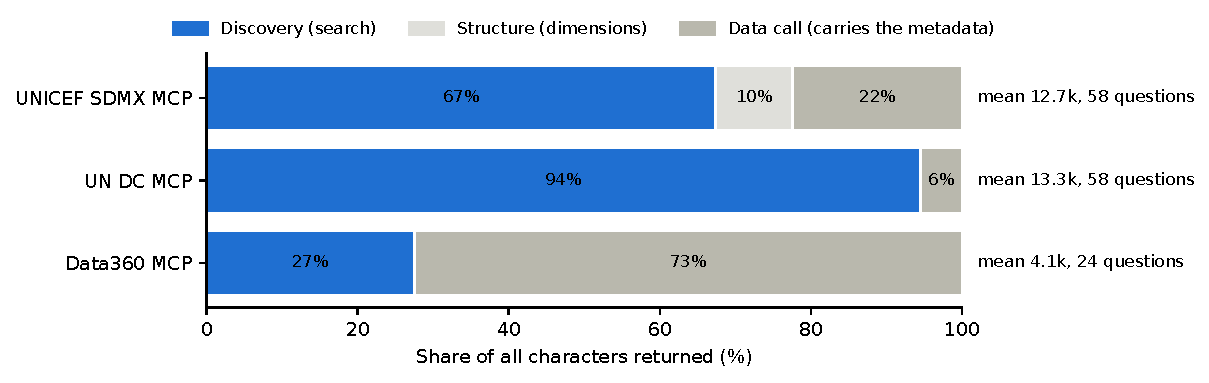
\includegraphics[width=\textwidth]{fig4_cost_components.pdf}
\caption{Share of all characters returned, by component of the answer; sector and country benchmark, fixed paths.}\label{fig:components}
\end{figure}

All three servers answered every Nigerian question. The warehouse and UN DC each answered \braAns{} of \braQ{} questions for Brazil and \somAns{} of \somQ{} for Somalia, missing the same ones because UN DC copies the warehouse's gaps. A question with no data costs the warehouse a median \noDataWh{} thousand characters and UN DC \noDataUn{} thousand, because UN DC's search filters by country first. UN DC's values matched the warehouse's in every common year on \unAgree{} of \unCommon{} answered questions; most of the rest are older releases. Its latest year was the same on \unLatSame{}, earlier on \unLatEarlier{} and later on \unLatLater{}. Data360 matched fully on \dAgree{} of \dCommon{} questions with common years, and its latest year was earlier on \dLatEarlier{} of \dLatN{}. Table~\ref{tab:sectors} gives the medians by sector.

\begin{table}[htbp]\centering\small
\caption{Median characters and share of the standard, by sector (unanswered questions included)}\label{tab:sectors}
\begin{tabularx}{\textwidth}{@{}Lcccc@{}}
\toprule
Sector & Questions & UNICEF SDMX MCP & UN DC MCP & Data360 MCP \\ \midrule
\csname @@input\endcsname generated/tab4_sectors.tex 
\bottomrule
\end{tabularx}
\end{table}

\subsection{Does the model or the effort level matter?}
Every setting answered all 12 questions, and every value reported for a year the warehouse holds was correct (Figure~\ref{fig:models}, Table~\ref{tab:models}). Of the \valuesRep{} year-values reported across the \sessions{} sessions, all \valuesOK{} for years the warehouse holds match it within rounding; the other is a year (2000) from a Data360 series the warehouse does not hold. Every reported number, including all \boundsOK{} uncertainty bounds, appears in the server's own responses. The reference has \refYears{} year-values per setting; the two missing in every row are a coverage gap in Data360's antenatal care series.

\begin{figure}[htbp]\centering
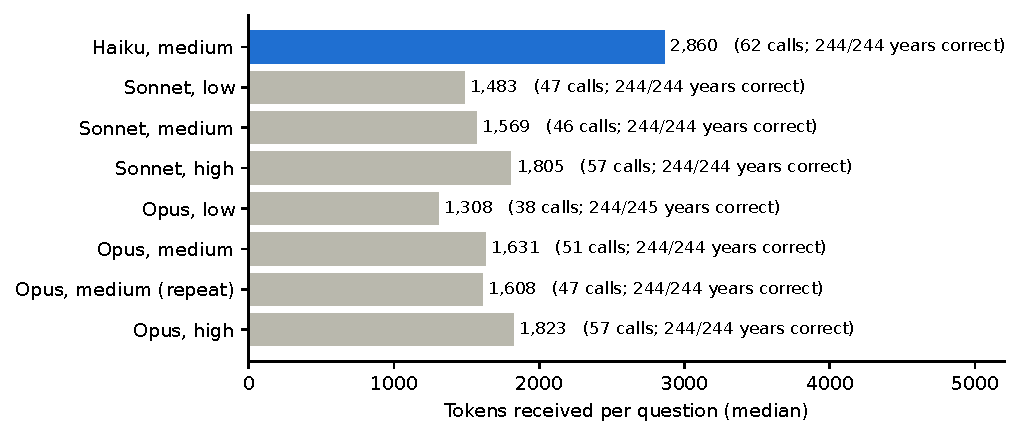
\includegraphics[width=\textwidth]{fig5_model_effort.pdf}
\caption{Tokens received per question (median), MCP calls and years correct, by model and effort setting; 12 questions per setting.}\label{fig:models}
\end{figure}

\begin{table}[htbp]\centering\small
\caption{Cost and accuracy by model and effort setting (12 questions each)}\label{tab:models}
\begin{tabularx}{\textwidth}{@{}Lcccccc@{}}
\toprule
Setting & \shortstack{Tokens sent\\per question} & \shortstack{Tokens received\\per question} & \shortstack{MCP\\calls} & \shortstack{Characters\\per question} & \shortstack{Years correct\\/ reported} & \shortstack{Metadata\\fields} \\ \midrule
\csname @@input\endcsname generated/tab5_models.tex 
\bottomrule
\multicolumn{7}{@{}l}{\footnotesize Medians per question, except MCP calls (total over 12 questions) and metadata fields (mean).}
\end{tabularx}
\end{table}

Completeness depended on which series the agent picked. Data360 holds antenatal care in two series: the Human Capital Project series starts in 2010 and misses 2003 and 2008; the Health, Nutrition and Population series ends in 2018 and misses the two latest surveys. Only Opus at low effort picked the second, so its latest value was from 2018.

Higher effort bought more calls, not better answers. For Opus, MCP calls rose from \callsOpusLow{} to \callsOpusMedium{} to \callsOpusHigh{} across low, medium and high effort, and tokens received from \recvOpusLow{} to \recvOpusMedium{} to \recvOpusHigh{} per question. Sonnet's tokens received rose in the same way (\recvSonnetLow{} to \recvSonnetHigh{}). Haiku made the most calls (\callsHaikuMedium{}) and generated the most tokens: \recvHaikuMedium{} per question, about \haikuRatio{} times Sonnet at medium effort.

The values were stable; the cost and the metadata were not (Table~\ref{tab:consistency}). Repeating Opus at medium effort reproduced the series and values in all \repSeries{} cells, but tokens sent per question changed by up to \repMax\%, and the median fell \repMed\%: about half the gap between low and high effort for Opus (+\opusEffort\%). The servers behaved deterministically: on UN DC, \unByteDiff{} of \unSigs{} repeated calls were byte-different only because JSON keys came back in a different order. One warehouse call, \texttt{get\_flow\_structure} for the child-mortality flow, returned \oversizedM{} million characters; the client refused it and the agent answered without it.

\begin{table}[htbp]\centering\small
\caption{Consistency and grounding}\label{tab:consistency}
\begin{tabularx}{\textwidth}{@{}Lr@{}}
\toprule
Check & Result \\ \midrule
\csname @@input\endcsname generated/tab6_consistency.tex 
\bottomrule
\end{tabularx}
\end{table}

\paragraph{Where the tokens go.} Tokens sent were about \sentPerRecv{} times tokens received. Most are not caused by the server: \baseShare\% is the client's own baseline of about \baseTok{} tokens re-sent with every request, and \cacheShare\% of all tokens sent were cache reads. Of what the server adds, its tool definitions dominate (Figure~\ref{fig:tokens}). Loading a server's tools adds about \schemaUn{} tokens (UN DC, six tools), \schemaWh{} (warehouse, 31 tools) or \schemaD{} (Data360, 16 tools) to every later request. Over a question of \reqMin{} to \reqMax{} requests that is \defMin{},000--\defMax{},000 tokens on average, against \respMin{},000--\respMax{},000 for all responses and reasoning together. Tool count alone does not set the cost: UN DC's six tools weigh almost as much as the warehouse's 31, because their descriptions are long. By characters, the largest items were Data360's \texttt{get\_metadata} (\dMetaChars{} per call) and UN DC's instruction file (\instrChars{}, read once per session); without it, UN DC needed a median of \charsUnNoFile{} thousand characters per question, against \charsWhAg{} thousand for the warehouse and \charsDAg{} thousand for Data360.

\begin{figure}[htbp]\centering
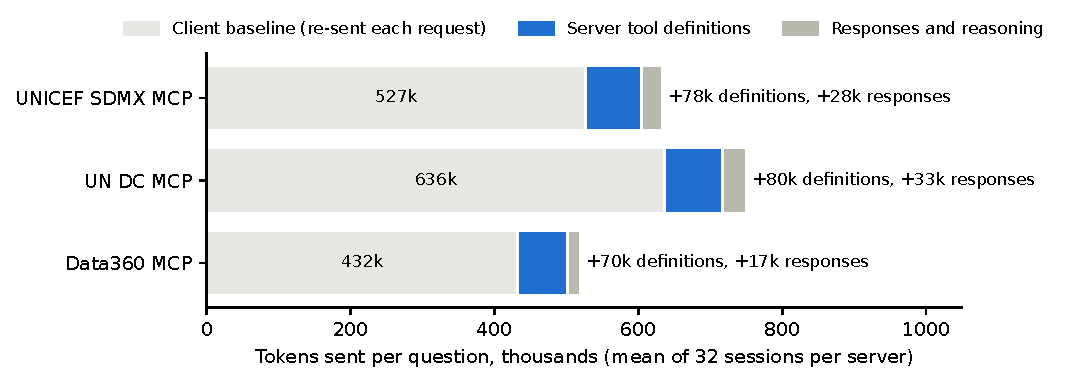
\includegraphics[width=\textwidth]{fig6_tokens_sent.pdf}
\caption{Tokens sent per question by component, mean of 32 sessions per server. Definitions: the jump in context when the server's tools load, times later requests.}\label{fig:tokens}
\end{figure}

% ======================================================================
\section{Policy implications}\label{sec:policy}

\subsection{For an official UNICEF MCP}
\begin{enumerate}
\item \textbf{Return values and the fifteen elements in one data call.} The metadata travels in the cheap part of the answer, and an agent rarely makes a second call. The gaps to close are a retrieval stamp (R2), a structured release and currency field (S6), licence and citation (S7), and status and bounds in the flows where they are empty (O3, O4), with the interval level stated.
\item \textbf{Make discovery compact.} Search should return a short ranked list of identifiers and names, filtered by country first, and leave definitions, units and flow lists to the data response; this is where \discWh\% of the warehouse's characters go, plus \structWh\% for structure.
\item \textbf{Keep the tool list short and its descriptions tight.} Tool definitions are re-sent with every request and in agentic use cost more tokens than the data. A small core set with advanced tools behind it would cut the largest server-attributable cost.
\item \textbf{Cap and page every response}, so that no single call can return \oversizedM{} million characters.
\item \textbf{Declare the response schema} through \texttt{outputSchema} and return conforming \texttt{structuredContent}.
\item \textbf{Test conformance and cost continuously}, with the fixed query sets and scoring scripts used here, reporting share of the standard, characters, tokens sent and received, accuracy and stability across repeated runs.
\end{enumerate}

\subsection{For republishers}
Pass through, never drop: almost all of UN DC's gaps are attributes the warehouse already publishes. Start with custodian attribution (S5) and release (S6), which answer the attribution concerns custodian agencies have raised and expose stale copies. Mark the canonical series: agents split between duplicate copies of the same series, and where the copies differ in coverage the choice changed the answer.

\subsection{For the statistical community}
The standard reuses SDMX and SDG attributes, so it asks custodians for nothing new. It can be tabled at the CCS-UN as the minimum any server that republishes custodian data should meet, with S5, S6 and S7 first, and proposed to the UN System Data Commons under UN80 Workstream 16.

\subsection{For evaluating agents on official data}
Monitor tokens sent and received separately: they differ by two orders of magnitude and respond to different design choices. Do not assume a smaller model is cheaper per answer, or that higher effort improves accuracy on well-specified questions. Repeat runs: run-to-run noise in cost was about half the effect of effort.

% ======================================================================
\section{Final remarks}\label{sec:final}

A modest standard of fifteen elements, built entirely from attributes the statistical system already defines, would let an agent reproduce, attribute, date and interpret every value, at no more than the cost of today's cheapest answers. The servers differ far more in what they pass through than in what they cost; cost is driven by search and by the tool list rather than by the data; and the model or effort level changes the cost but not the values. The design of the server, not the choice of model, decides whether an answer is complete and attributable.

\paragraph{Limitations.} The agentic benchmark covers four series for one country with one repeat; the sector benchmark covers three countries; both are snapshots of servers that change. The warehouse is both a server under test and the reference, so a value it has wrong would not be detected. The client's baseline is specific to the agent harness used, although the tool-definition and response components are not. Claude Fable 5.1 and other model families were not tested. The prompt was well specified; open-ended or ambiguous questions may separate models more. Partial scores involve judgement, although the automated rules reproduce the hand scores of the pilot.

\paragraph{Next steps.} Run the agentic benchmark with at least three repeats per setting, on more countries and open-ended questions; run all three benchmarks against the prototype of the official UNICEF MCP before and after implementing the standard and a compact search; and publish the query sets and scoring as a conformance test any republishing server can run.

\section*{Reproducibility}
Every number in the text is a macro written by \texttt{paper/code/assets.py} from the analysis outputs, every table is generated and every figure is drawn from the same files; \texttt{make all} rebuilds the analysis, the assets and this PDF from the saved server responses and agent transcripts in the repository. Collection (querying live servers with agents) is documented but not re-executed by \texttt{make}, since the servers change.

\bibliographystyle{plainnat}
\bibliography{references}
\nocite{*}
\end{document}
